\chapter{Revue de la Littérature et Concepts de Base}

\section{Introduction}
Dès \textbf{1997}, le potentiel du \textbf{data mining} pour améliorer les problèmes dans le domaine médical avait été identifié par l'Organisation mondiale de la santé (\textbf{OMS}) (Gulbinat, 1997). L'utilité de la détection de connaissances à partir des dépôts de données médicales a été soulignée par l'OMS, car elle bénéficie au diagnostic médical et à la prédiction. Le data mining est un processus de découverte de connaissances utiles à partir de bases de données pour construire une structure (c'est-à-dire un modèle ou un schéma) qui peut interpréter de manière significative les données. Le data mining est le processus de découverte de schémas et de connaissances intéressants à partir d'une grande quantité de données (Han et al., 2001). Le data mining utilise de nombreuses techniques d'apprentissage automatique pour découvrir des schémas cachés dans les données. Ces techniques peuvent être réparties en trois catégories principales : les techniques d'\textbf{apprentissage supervisé}, les techniques d'\textbf{apprentissage non supervisé} et les techniques d'\textbf{apprentissage semi-supervisé} (Huang al., 2014). Voir figure \ref{fig:machinelearningtype}. Les systèmes experts développés par des techniques d'apprentissage automatique peuvent être utilisés pour aider les médecins dans le \textbf{diagnostic} et la \textbf{prédiction des maladies} (Kononenko, 2001). En raison de l'importance du diagnostic des maladies pour l'humanité, plusieurs études ont été menées sur le développement de méthodes pour leur classification~\cite{Analytical2017Meh}.

\section{Apprentissage Automatique}
Depuis leur évolution, les humains ont utilisé de nombreux types d'outils pour accomplir diverses tâches de manière plus simple. La créativité du cerveau humain a conduit à l'invention de différentes machines. Ces machines ont facilité la vie humaine en permettant aux gens de répondre à divers besoins de la vie, y compris le voyage, les industries et l'informatique. Et l'apprentissage automatique en fait partie. Selon Arthur Samuel, l'\textbf{apprentissage automatique} est défini comme le domaine d'étude qui donne aux ordinateurs la capacité d'apprendre sans être explicitement programmés. \textit{Arthur Samuel} était célèbre pour son programme de jeu de dames. L'apprentissage automatique (\textbf{ML}) est utilisé pour apprendre aux machines comment gérer les données de manière plus efficace. Parfois, après avoir examiné les données, nous ne pouvons pas interpréter les informations extraites des données. Dans ce cas, nous appliquons l'apprentissage automatique. Avec l'abondance des ensembles de données disponibles, la demande pour l'apprentissage automatique est en hausse. De nombreuses industries appliquent l'apprentissage automatique pour extraire des données pertinentes. Le but de l'apprentissage automatique est d'\textit{apprendre à partir des données}~\cite{Machine2020Batta}.
\begin{figure}[!h]
	\centering
	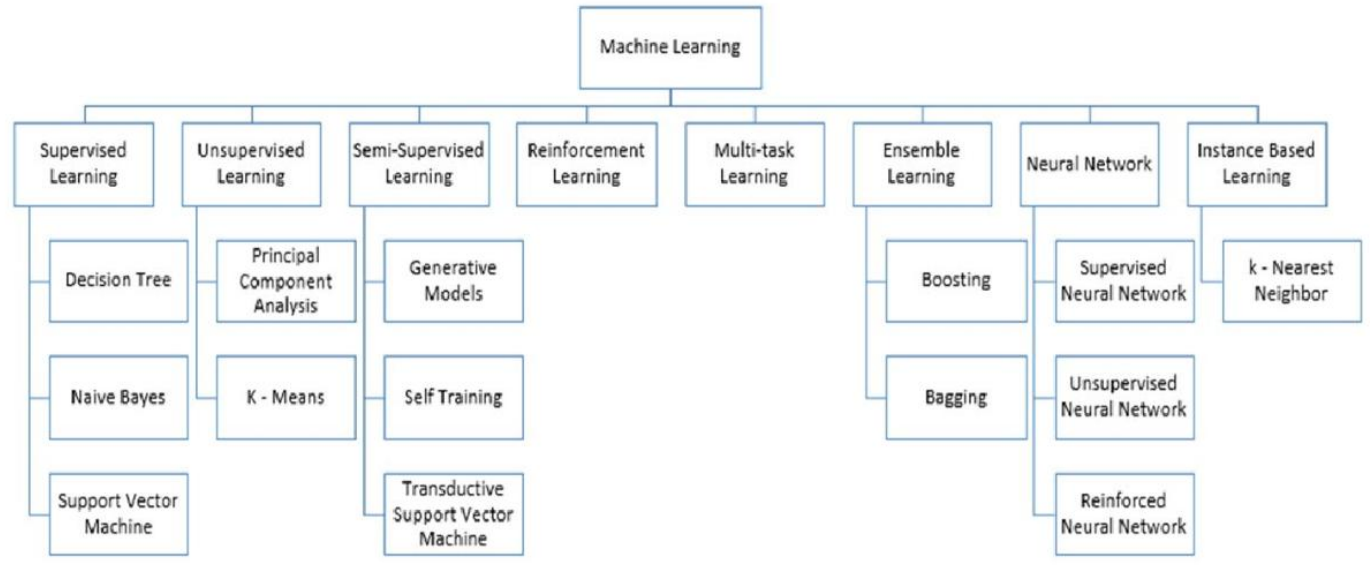
\includegraphics[width=0.7\linewidth]{images/machineLearningType}
	\caption{}
	\label{fig:machinelearningtype}
\end{figure}

\subsection{Techniques d'Apprentissage Automatique}
Voici un aperçu rapide de certains des algorithmes couramment utilisés en apprentissage automatique (ML)
\subsubsection{Apprentissage Supervisé}
Les algorithmes d'\textbf{apprentissage supervisé} sont ceux qui nécessitent une assistance externe. L'ensemble de données d'entrée est divisé en ensemble d'entraînement et ensemble de test. L'ensemble d'entraînement a une variable de sortie qui doit être prédite ou classée. Tous les algorithmes apprennent un certain type de schémas à partir de l'ensemble d'entraînement et les appliquent à l'ensemble de test pour la prédiction ou la classification. Le flux de travail des algorithmes d'apprentissage supervisé est donné dans la figure \ref{fig:suppervisedlearning} ci-dessous~\cite{Machine2020Batta}.

Exemple d'apprentissage supervisé :
\begin{itemize}
	\item \textbf{Arbre de Décision} : est un graphe pour représenter les choix et leurs résultats sous forme d'arbre.
	\item \textbf{Naïve Bayes} : C'est une technique de classification basée sur le théorème de Bayes avec une hypothèse d'indépendance entre les prédicteurs. En termes simples, un classificateur Naïve Bayes suppose que la présence d'une caractéristique particulière dans une classe est indépendante de la présence de toute autre caractéristique.
\end{itemize}
\begin{figure}[!h]
	\centering
	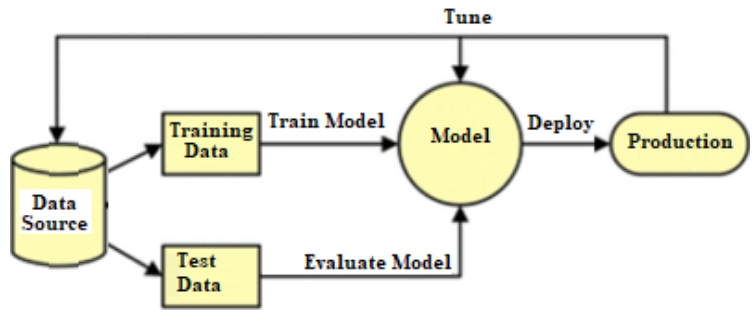
\includegraphics[width=0.6\linewidth]{images/supervisedlearning}
	\caption{Flux de travail de l'apprentissage supervisé}
	\label{fig:suppervisedlearning}
\end{figure}
\newpage
\subsubsection{Apprentissage Non Supervisé}
Contrairement à l'apprentissage supervisé ci-dessus, il n'y a pas de réponses correctes et il n'y a pas de professeur. Les algorithmes sont laissés à leurs propres dispositifs pour découvrir et présenter la structure intéressante dans les données. Les algorithmes d'apprentissage non supervisé apprennent quelques caractéristiques à partir des données. Lorsque de nouvelles données sont introduites, elles utilisent les caractéristiques apprises précédemment pour reconnaître la classe des données. Il est principalement utilisé pour le \textit{clustering} et la réduction des \textit{features}~\cite{Machine2020Batta}.

Exemple d'apprentissage non supervisé :
\begin{itemize}
	\item \textbf{Clustering K-means} : est l'un des algorithmes d'apprentissage non supervisé les plus simples qui résout le problème bien connu du clustering. La procédure suit une manière simple et facile de classer un ensemble de données donné par un certain nombre de clusters.
\end{itemize}

\begin{figure}[!h]
	\centering
	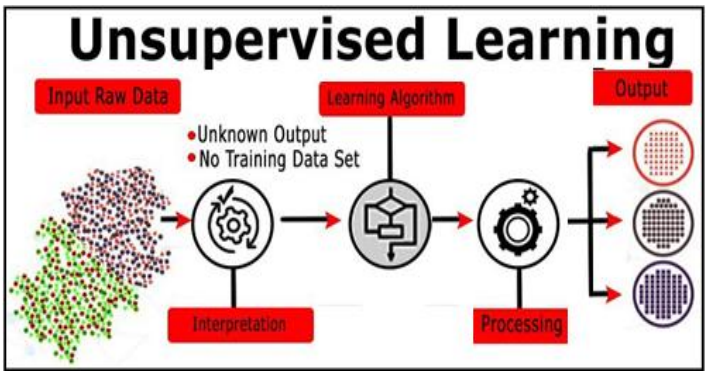
\includegraphics[width=0.6\linewidth]{images/unsupervisedlearning}
	\caption{Apprentissage Non Supervisé}
	\label{fig:unsupervisedlearning}
\end{figure}

\subsubsection{Apprentissage Semi-Supervisé}
L'\textbf{apprentissage semi-supervisé} est une combinaison des méthodes d'apprentissage \textit{supervisé} et \textit{non supervisé}. Il peut être fructueux dans ces domaines de l'apprentissage automatique et du data mining où les données non étiquetées sont déjà présentes et obtenir les données étiquetées est un processus fastidieux~\cite{Machine2020Batta}. 
\subsubsection{Apprentissage par Ensemble}
L'\textbf{apprentissage par ensemble} est le processus par lequel plusieurs \textbf{modèles}, sont générés et combinés stratégiquement pour résoudre un problème particulier d'intelligence computationnelle. L'apprentissage par ensemble est principalement utilisé pour améliorer les performances d'un modèle ou réduire la probabilité de sélectionner un modèle médiocre~\cite{Machine2020Batta}. 

Exemple d'apprentissage par ensemble :
\begin{itemize}
	\item \textbf{Boosting} : Le terme "\textit{Boosting}" fait référence à une famille d'algorithmes qui convertit les apprenants faibles en apprenants forts. Le boosting est une technique d'apprentissage par ensemble utilisée pour réduire le biais et la variance.
	\item \textbf{Bagging} : est appliqué lorsque la précision et la stabilité d'un algorithme d'apprentissage automatique doivent être augmentées. Il est applicable en classification et en régression. Le bagging réduit également la variance et aide à gérer le surapprentissage.
\end{itemize}

\subsection{Applications de l'Apprentissage Automatique à l'Épidémiologie}
\subsection{Avantages et Limites de l'Apprentissage Automatique}

\section{Deep Learning}
\subsection{Définition et Concepts Fondamentaux}
\subsection{Réseaux de Neurones Artificiels}
\subsubsection{Perceptron Multicouche (MLP)}
\subsubsection{Réseaux de Neurones Convolutifs (CNN)}
\subsubsection{Réseaux de Neurones Récurrents (RNN)}
\subsection{Applications du Deep Learning à l'Épidémiologie}
\subsection{Avantages et Limites du Deep Learning}

\section{Ensemble Regression Learning}
\subsection{Définition et Concepts Fondamentaux}
\subsection{Techniques d'Ensemble Learning}
\subsubsection{Bagging}
\subsubsection{Boosting}
\subsubsection{Stacking}
\subsection{Applications de l'Ensemble Regression Learning}
\subsection{Avantages et Limites de l'Ensemble Regression Learning}

\section{Conclusion}
